\section{Results}
\label{sec:results}
Make some awesome plots from the topics over time, rank by (upvotes | comments | number of articles published)

\begin{figure}[H]
	\caption{Topic group sizes}
	\label{fig:topicsizes}
	\centering
	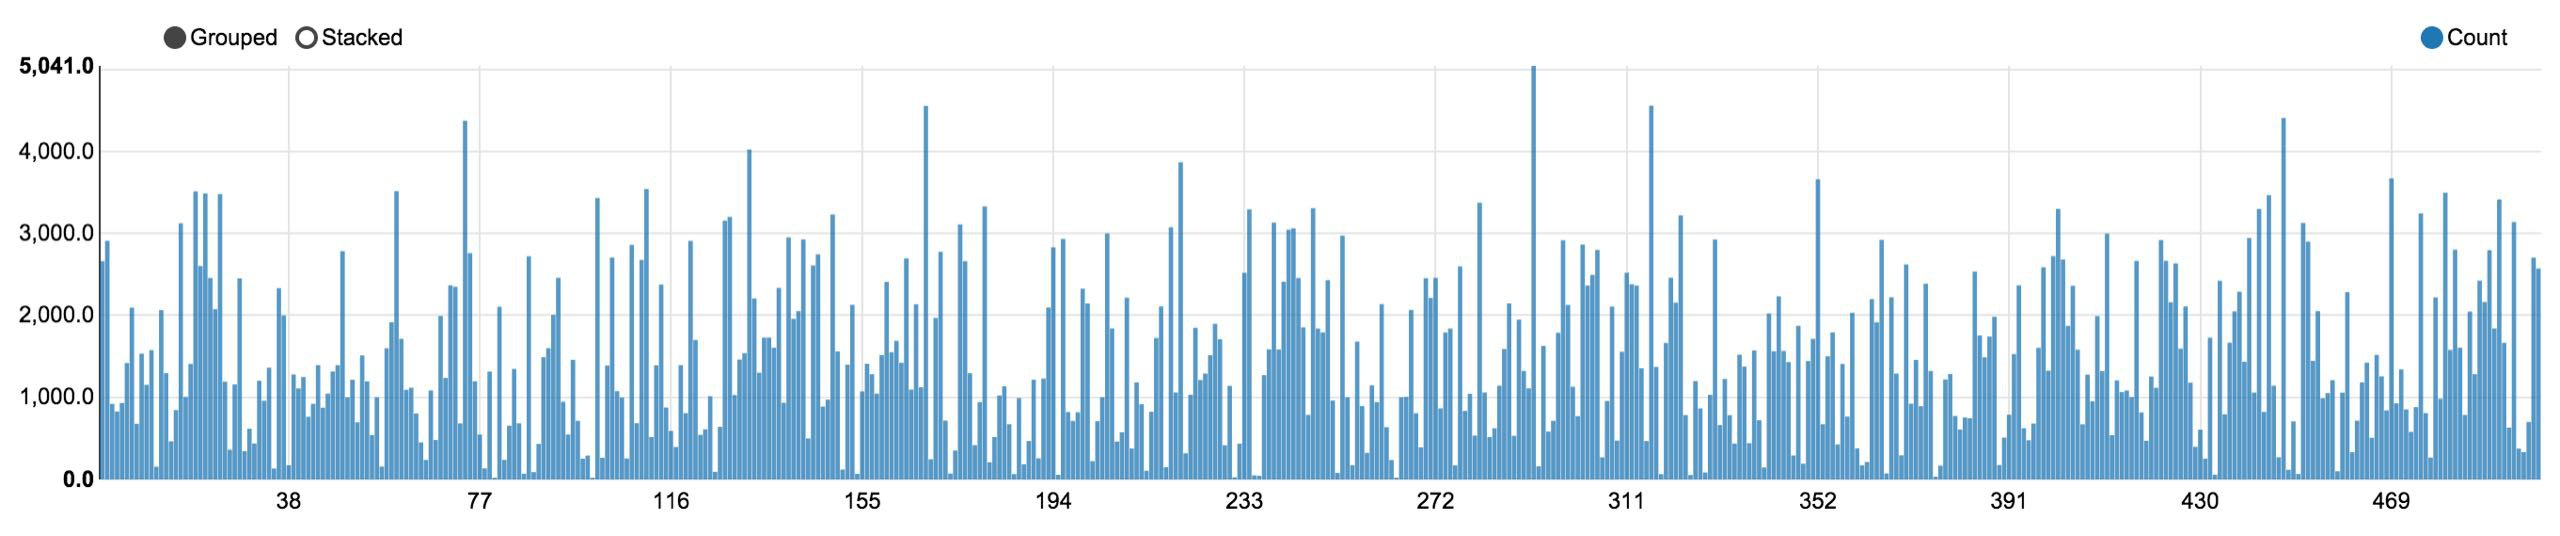
\includegraphics[width=14cm]{topicsizes}
\end{figure}

\subsection{Popularity plots}
In this section, we will show some awesome plots of how the popularity of various topics changed over time.

\begin{figure}[H] % Topic 412
	\caption{Popularity of Docker, CoreOS, etcd, containers, OpenStack}
	\label{fig:trend_docker}
	\centering
	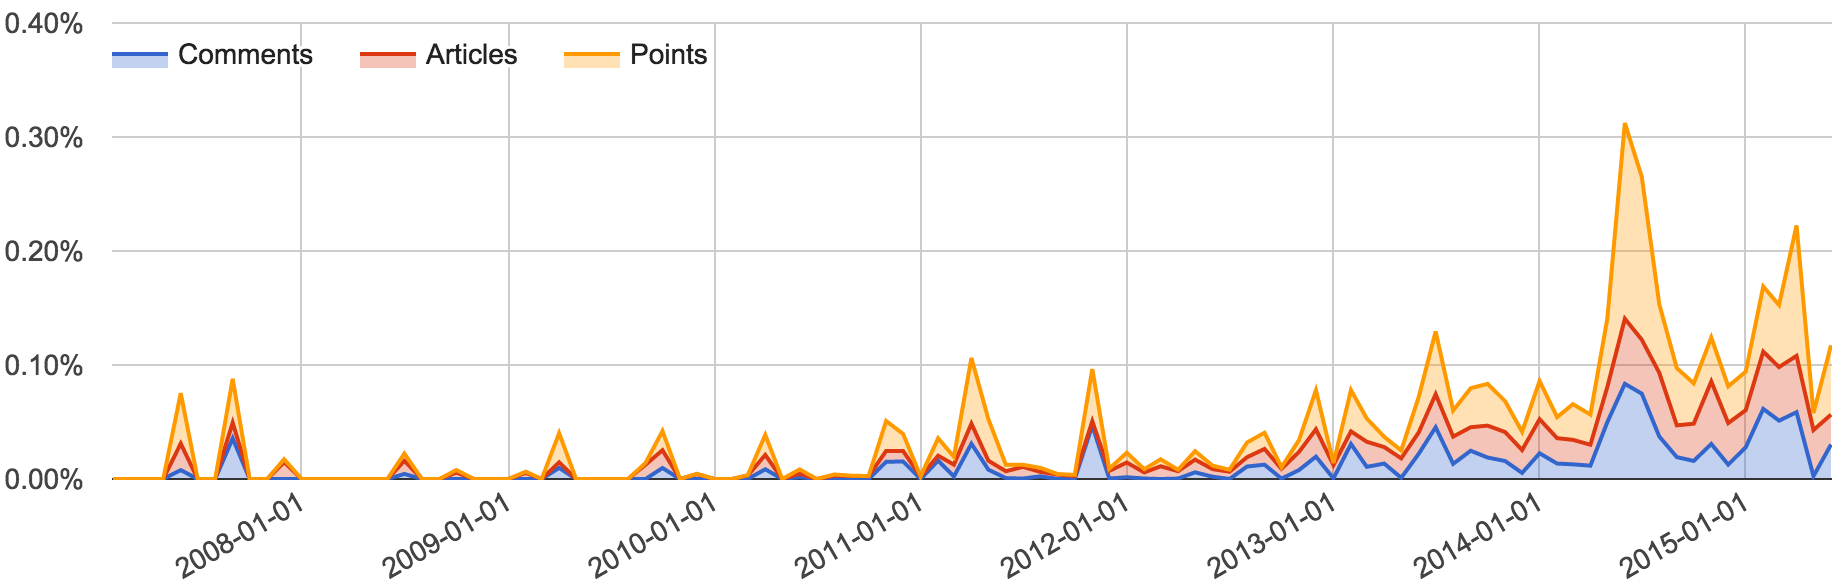
\includegraphics[width=14cm]{topic_trends/docker_relative}
	% docker coreos etcd images:containers openshift mesos deis openstack orchestration dokku
\end{figure}
We start the overview with a trend plot (figure~\ref{fig:trend_docker}) of a new and upcoming technique: containerization. Docker and CoreOS were released in March resp. October 2014 and before that, containerization was already used as a term for seperating Linux processes. The trends show how Docker started gaining some real traction within half a year and is really booming in the first half of 2015.

\begin{figure}[H] % Topic 383
	\caption{Popularity of Elon Musk, SpaceX, Tesla, Hyperloop}
	\label{fig:trend_elon}
	\centering
	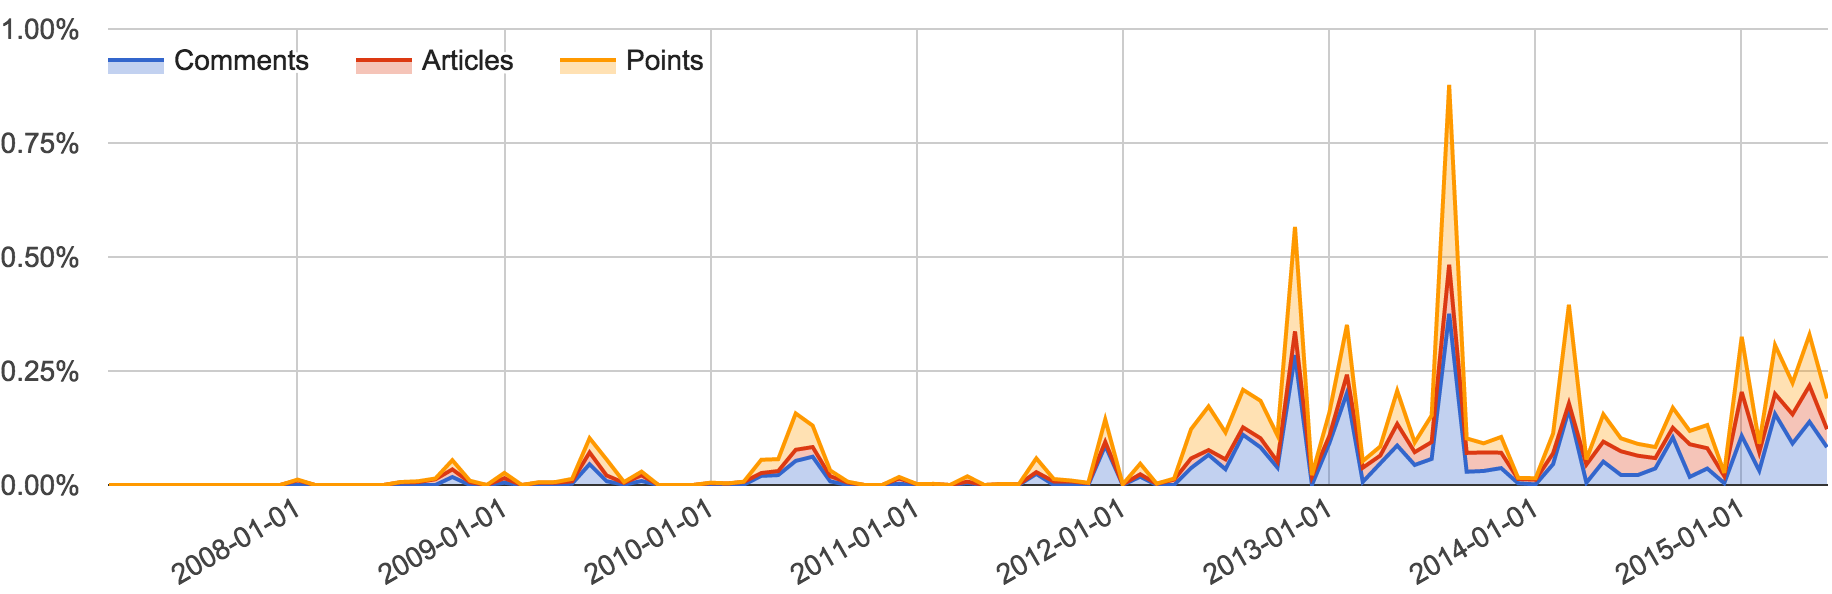
\includegraphics[width=14cm]{topic_trends/elon_relative}
	% elon musks spacex musk's tesla hyperloop test track musk
\end{figure}
\textbf{Something about Elon's awesome projects :)}

\begin{figure}[H] % Topic 79
	\caption{Popularity of keynote, Apple, live, @scale, conference}
	\label{fig:trend_keynote}
	\centering
	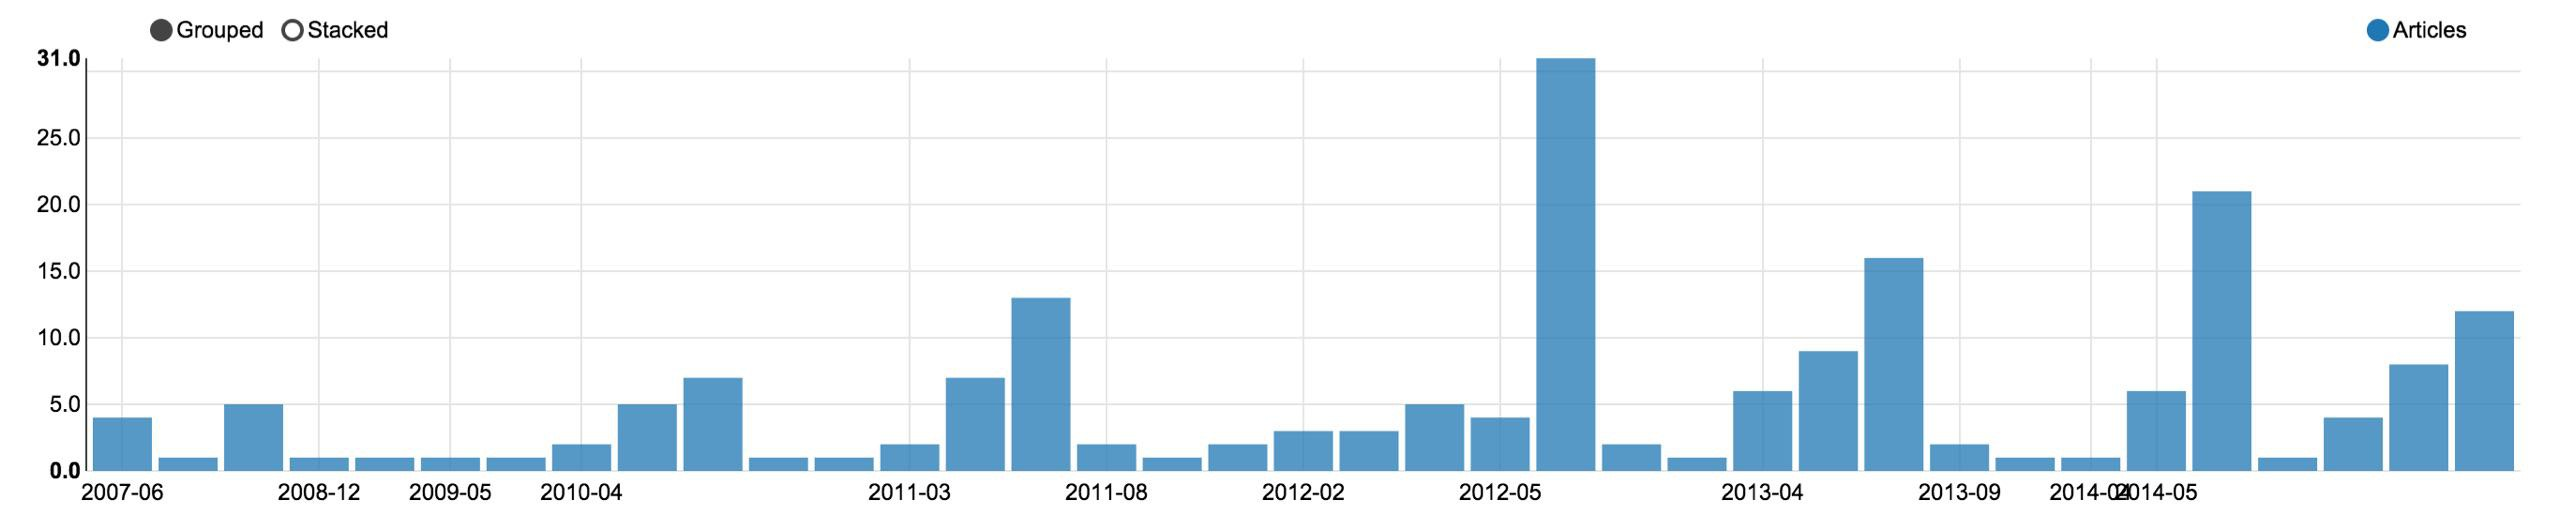
\includegraphics[width=14cm]{topic_trends/keynote}
	% keynote apple live yesterday's apple's @scale apple developers conference keynotes conference macworld
\end{figure}
In the popularity charts of keynote-related topics (figure~\ref{fig:trend_keynote}), one can see patterns of three months of increasing popularity. The highest point is always the month in which an Apple keynote took place; the two months before usually have rumours about what new products will be introduced.

The big spike halfway 2012 marks the announcement of Siri, Apple's articifial intelligence personal assistant.

Unfortunately, Hacker News started after the release of the iPhone (January 2007; one month too early), so we cannot see the data for that release.

\begin{figure}[H] % Topic 579
	\caption{Popularity of Steve Jobs, Wozniak, imagineers}
	\label{fig:trend_jobs}
	\centering
	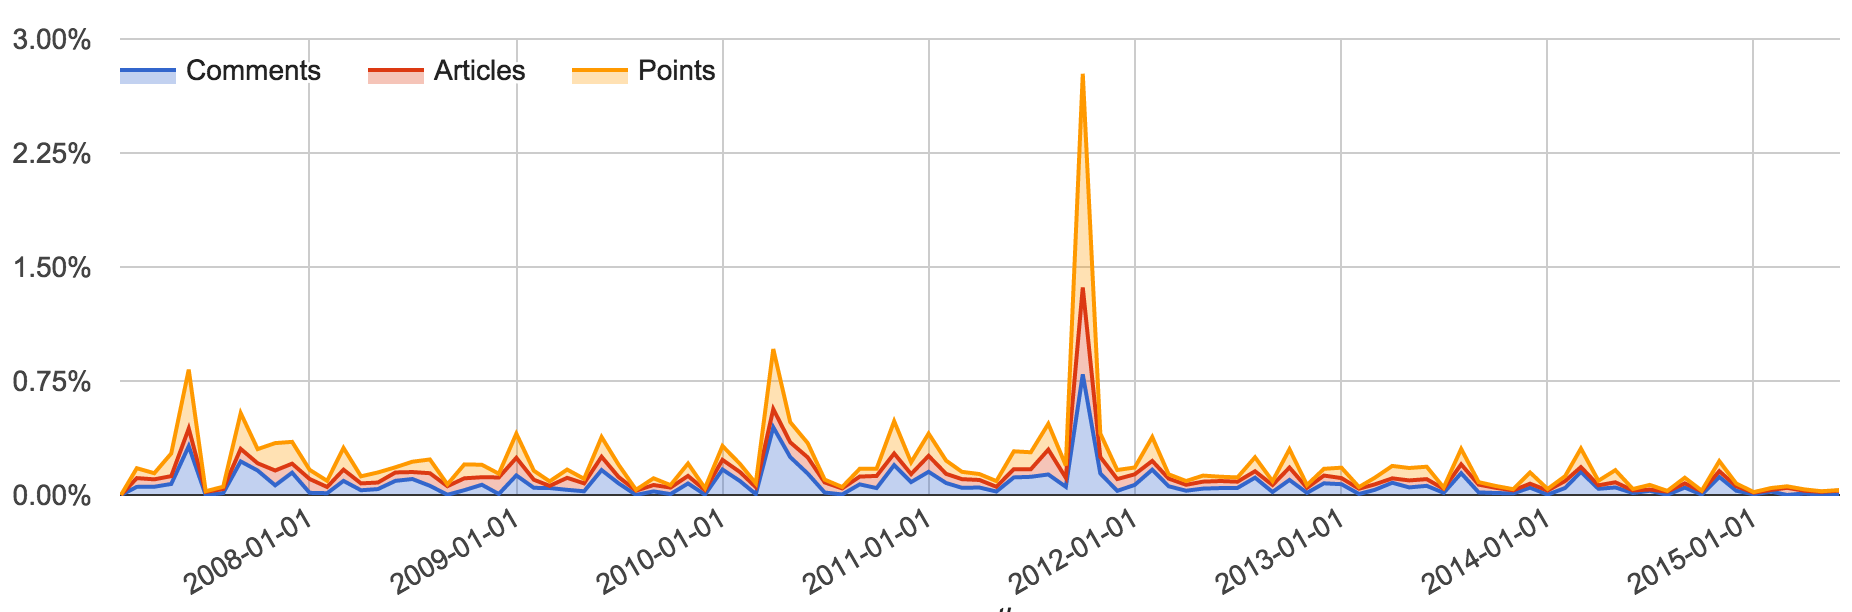
\includegraphics[width=14cm]{topic_trends/jobs_relative}
	% jobs wozniak woz jobs. steve steves jobs's jobssteve imagineers wozs
	% Interesting: Tim Cook is not in this cluster, and his coming out is therefore not visible in this graph
\end{figure}

On the topic of Apple: not only it's products spark the interest of the Hacker News community; it's former CEO also had a big impact in the community. We show figure~\ref{topic_trends/jobs} to indicate the enormous impact the death of Steve Jobs had. He shares this topic group with his co-founder Steve Wozniak, but the news of his death (October 5th, 2011) dwarfs all other events in Hacker News history.

\begin{figure}[H] % Topic 17
	\caption{Popularity of Raspberry Pi, Kindleberry}
	\label{fig:trend_raspberry}
	\centering
	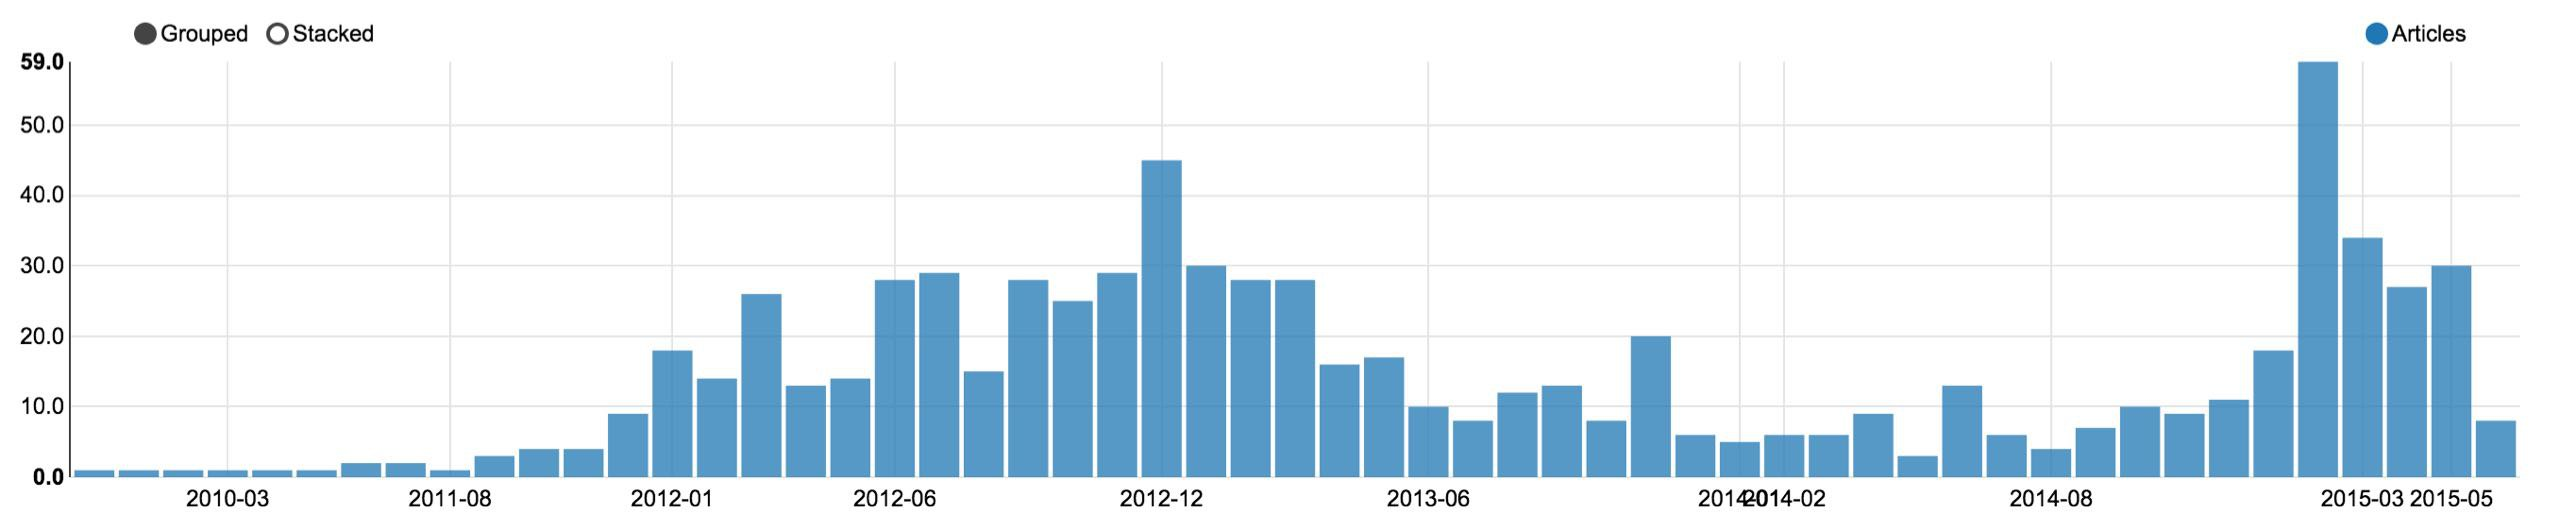
\includegraphics[width=14cm]{topic_trends/raspberry}
	% raspberry pi's kindleberry pis navio+ motherbone-tm-pione-tm- piface razberry rpi raspberrypi
\end{figure}

\begin{figure}[H] % Topic 70
	\caption{Popularity of Edward Snowden, Wistleblower, leaks, Reddit}
	\label{fig:trend_snowden}
	\centering
	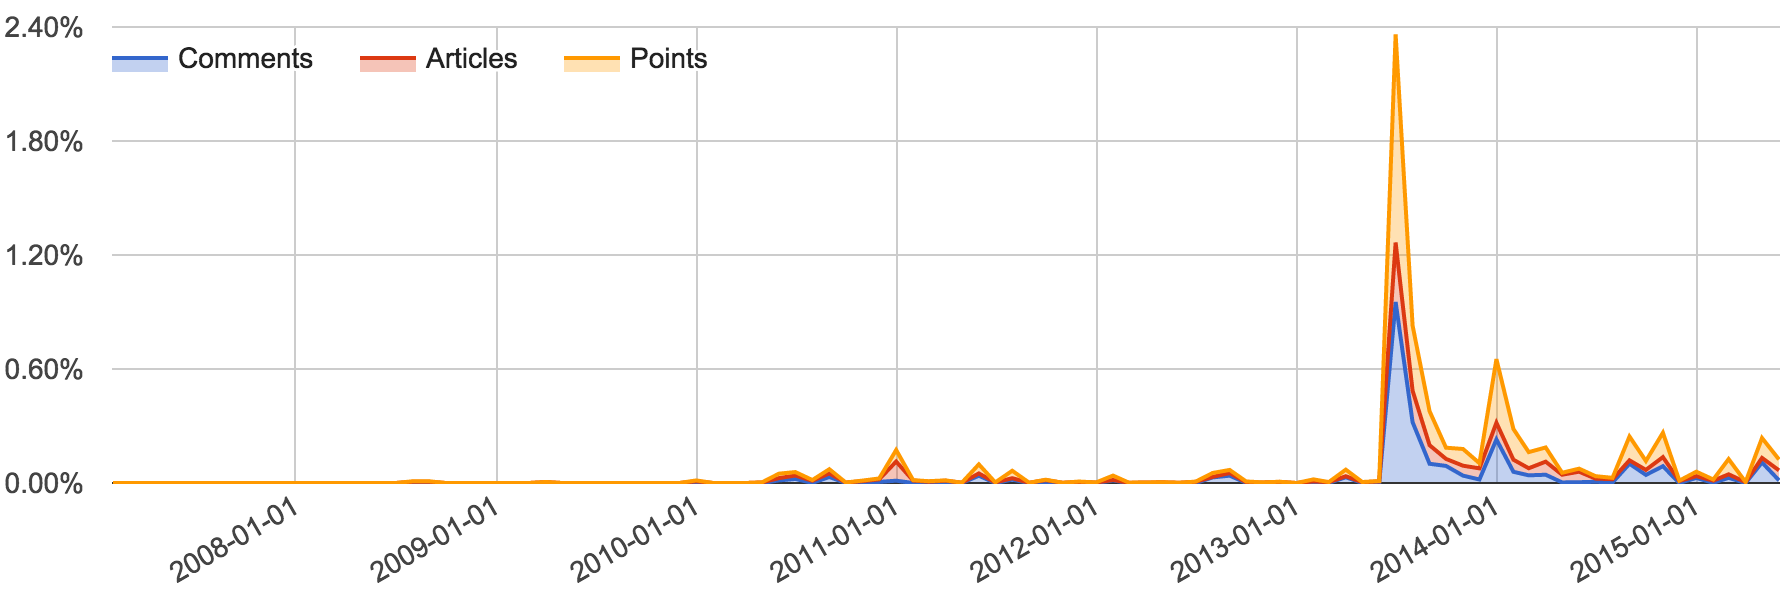
\includegraphics[width=14cm]{topic_trends/snowden_relative}
	% edward whistleblower contractor-turned-whistleblower snowden.the snowden's leaker snowdens reddit.comsubmitted snowden. snowden.in
\end{figure}
\lipsum[1]
